\section{3D-HybridEngine} \label{sec:hybrid_engine}
\begin{figure}[t]
    \centering
    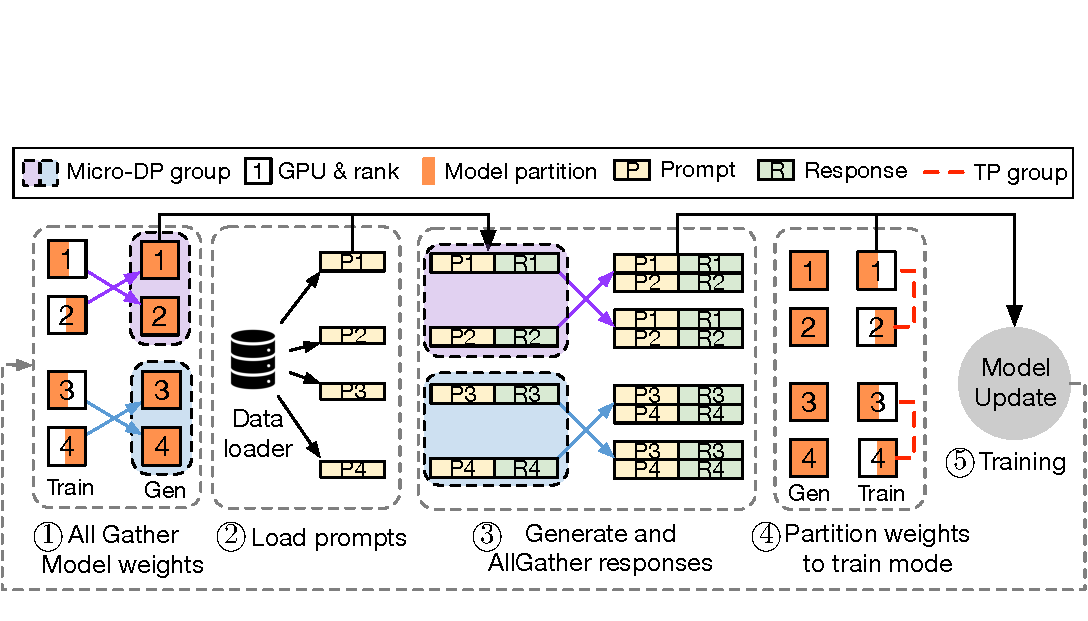
\includegraphics[width=\linewidth]{figs/fig_hybrid_one_iter_2.pdf}
    \vspace{-5mm}
    \caption{3D-HybridEngine workflow in one RLHF iteration. 4 GPUs are used for actor training and generation. 1-2-2 ($p$-$t$-$d$) parallel groups are used in training and 1-1-2-2 ($p_g$-$t_g$-$d_g$-$d$) parallel groups are used in generation.
    }
    \label{fig:hybrid_one_iter}
    \vspace{-2mm}
\end{figure}

We design the \textit{3D-HybridEngine} %
to support efficient training and generation of the actor model, %
targeting significant RLHF throughput improvement.

\subsection{Parallel Groups}%

To eliminate redundant actor model copies, we advocate deploying actor training and generation stages %
on the same set of devices, $N_a$ GPUs allocated to the actor, and execute them sequentially on the same copy of actor model weights. Nonetheless, actor training and generation may well adopt different 3D parallelism strategies, i.e., the generation stage typically requires smaller TP and PP sizes but a larger DP size, than the training stage (\textsection\ref{sec:hybrid_motivation}). 3D-HybridEngine enables efficient model parameter resharding between actor training and generation across the same set of devices in this context. 

Let $p$-$t$-$d$ denote 3D parallel groups constructed for %
actor training, corresponding to the set of GPUs to host $p$ pipeline stages, $t$ tensor shards, and $d$ model replicas~\cite{narayanan2021efficient}. 3D-HybridEngine builds different parallel groups for actor training and generation, according to their different 3D parallelism strategies, respectively. We use $p_g$, $t_g$, and $d_g$ to denote the size of generation pipeline parallel group, generation tensor parallel group, and micro data parallel group, respectively, 
in the generation stage.  
$d_{g}$ indicates the ratio %
of model replica number in generation over that in training, i.e., each DP replica in training becomes $d_{g}$ micro DP replicas, to process $d_{g}$ microbatches of prompts and responses. We have $N_a$=$p$$\times$$t$$\times$$d$=$p_g$$\times$$t_g$$\times$$d_g$$\times$$d$ such that $d_{g} = \frac{pt}{p_{g}t_{g}}$. %
The micro DP groups are employed exclusively in actor generation stage to render a larger DP size for full device utilization.
The generation parallel groups are denoted by $p_g$-$t_g$-$d_g$-$d$. %


\subsection{3D-HybridEngine Workflow}
Between actor training in iteration $i$ of RLHF and actor generation in iteration $i+1$, the actor model parameters need to be resharded and prompts data to be distributed,
following the parallel group configurations in the two stages.
In iteration $i+1$ of RLHF, %
3D-HybridEngine gathers the actor model parameters updated in iteration $i$ (step $\textcircled{1}$ in Figure~\ref{fig:hybrid_one_iter}), for generation within each micro DP group. Then, the batch of prompts are loaded to each model replica (step $\textcircled{2}$), which generates responses (Generation stage of RLHF). 
Following this, 3D-HybridEngine performs an all-gather operation on the generation results within each micro DP group (step $\textcircled{3}$), and re-partitions %
model parameters according to the 3D parallelism for actor training %
(step $\textcircled{4}$). 
With model weights, prompts and responses correctly re-distributed, %
the loss of the actor model is computed and actor model weights are updated following the RLHF algorithm %
(step $\textcircled{5}$) - actor training stage of iteration $i+1$.


















\begin{figure}[t]
    \centering
    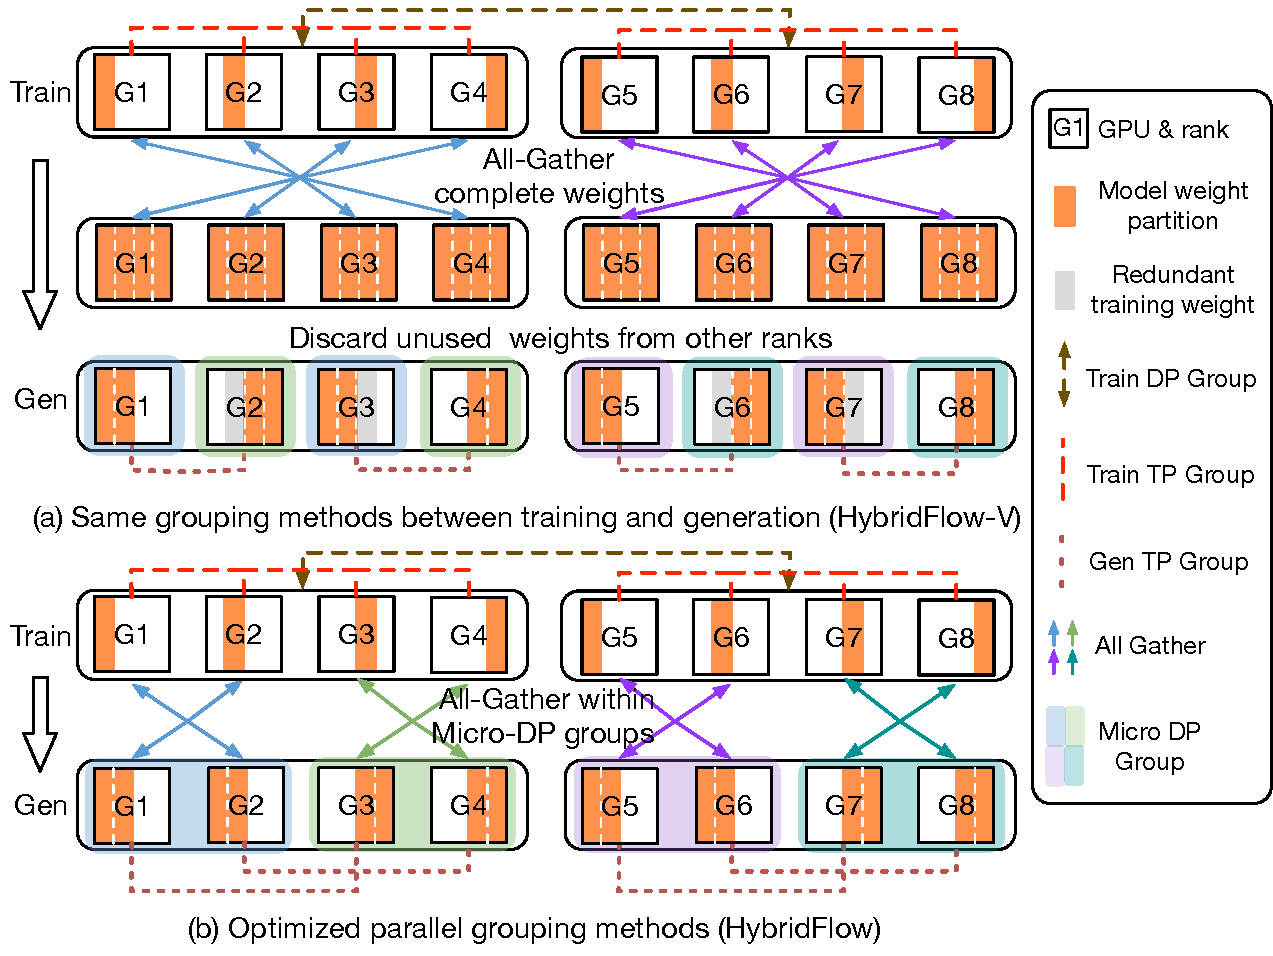
\includegraphics[width=\linewidth]{figs/fig_hybrid_comm_compare.pdf}
    \vspace{-5mm}
    \caption{Model weights resharding. 2 machines each with 4 GPUs are used for actor training and generation. %
    }
    \label{fig:comm_naive}
    \vspace{-3mm}
\end{figure}

\vspace{-1mm}
\subsection{Zero redundancy model resharding} \label{sec:hybrid_zero_redundancy}
Parallel grouping methods in 3D parallelism are typically as follows: %
PP and TP groups are formed by assigning consecutive ranks to pipeline stages and tensor shards, respectively; DP groups are constructed by selecting ranks at regular intervals, determined by the product of PP size and TP size. 
In Figure~\ref{fig:comm_naive}(a), actor training uses 3D parallel groups, 1-4-2: there is one PP group for all GPUs (for illustration clarify);
the TP groups are [G1, G2, G3, G4], [G5, G6, G7, G8], and the DP groups are [G1, G5], [G2, G6], [G3, G7], [G4, G8]. %
Suppose the same parallel grouping methods are used but with different parallel sizes, e.g., 1-2-2-2 for generation in Figure~\ref{fig:comm_naive}(a).
During the transition from training to generation, 3D-HybridEngine applies all-gather operations among the model 
parallel groups to aggregate all parameters, and then retain only a subset of model weights on each device for its generation, according to the parallel groups the device belongs to.
On some GPUs (e.g., G2, G3, G6, G7), there is no overlap between training and generation model weights, and separate memory is needed to maintain weights for subsequent training as well (grey boxes in Figure~\ref{fig:comm_naive}(a)).%
We call the system \sysname-V, when 3D-HybridEngine uses the above {vanilla} parallel grouping methods in 
{the two stages.}





We further design a new parallel grouping method for 3D-HybridEngine to use in the generation stage, that eliminates the redundancy in weights storage and leads to minimal memory footprint and communication due to actor model resharding between training and generation. %
Specifically, we form generation TP and PP groups by selecting ranks at regular intervals, determined by $\frac{t}{t_g}$ and $\frac{p}{p_g}$, and construct micro DP groups by sequentially assigning ranks along the generation TP or PP dimensions.
In Figure~\ref{fig:comm_naive}(b), 1-2-2-2 parallel groups are used in generation: the generation TP groups are [G1, G3], [G2, G4], [G5, G7], [G6, G8]; %
and the micro DP groups are [G1, G2], [G3, G4], [G5, G6], [G7, G8].
This strategic rearrangement of generation parallel groups leads to overlap between training and generation model weights on each device, enabling reuse of training weights during generation and
\textit{zero redundancy} in device memory usage due to model resharding. In addition, 3D-HybridEngine conducts several all-gather operations concurrently, one within each micro DP group, leading to significantly reduced 
communication overhead.






\begin{table}
\caption{%
Transition overhead between training \& generation
}
\vspace{-2mm}
\resizebox{\linewidth}{!}{
\begin{tabular}{c|c|c|c}
\toprule
& DS-Chat& \sysname-V & \sysname \\ 
\midrule
\makecell{Comm. Vol} & $\frac{tpd - 1}{tpd}M$ & $\frac{tp - 1}{tp}M$ & $\frac{tp-t_gp_g}{t_gp_gtp}M$ \\ 
\midrule
\makecell{Peak Mem.}   & $M$   & $M$  & $\frac{1}{t_gp_g}M$ \\ \midrule
Redundancy& $\frac{1}{tpd}M$ & $\frac{1}{tp}M$ & 0 \\ \bottomrule                
\end{tabular}
}
\label{tab:comm_mem_analysis}
\vspace{-3mm}
\end{table}
\subsection{Transition overhead} \label{sec:hybrid_comm_mem}


In Table~\ref{tab:comm_mem_analysis}, we compare communication overhead and memory footprint during the transition between training and generation stages, among different actor engine designs. %
We assume model size of the actor is $M$ and $N_a$ GPUs are used for its training and generation. The actor engine in DeepSpeed-Chat conducts an all-gather operation across all GPUs during transition; \sysname-V performs this all-gather within training TP and PP groups. The communication volumes for these operations are %
$\frac{N_a-1}{N_a}M=\frac{tpd - 1}{tpd}M$ for DeepSpeed-Chat %
 and $\frac{tp-1}{tp}M$ for \sysname-V, calculated following~\cite{chan2007collective}. 
Both engines aggregate all model parameters in each GPU's memory before subsequently partitioning model states according to the generation parallel groups, resulting in a peak memory usage of model parameters $M$. %
As they cannot reuse training weights during generation on some GPUs, training weights need to be maintained on them, %
amounting to $\frac{1}{tpd}$ and $\frac{1}{tp}$ redundant memory consumption, respectively.






With our parallel grouping method for the generation stage, \sysname{} confines the all-gather operation within each micro DP group. 
The communication overhead is reduced to $\frac{d_g - 1}{tp}M = \frac{tp-t_gp_g}{t_gp_gtp}M$. %
Each GPU only needs to collect remote parameters within its micro DP group and can reuse the training weights in generation. Therefore, the peak memory usage of model parameters in \sysname{} precisely matches the model partition size on each GPU in generation, eliminating any redundancy in %
GPU memory usage.










